\documentclass[11pt, oneside]{article}
\usepackage{geometry}
\geometry{a4paper} 
\usepackage{graphicx}
\usepackage{amssymb}


\title{Is Florida getting warmer?}
\author{Xuan Wang}
\date{Oct 2022}

\begin{document}
\maketitle


\section{Results}
\begin{center}
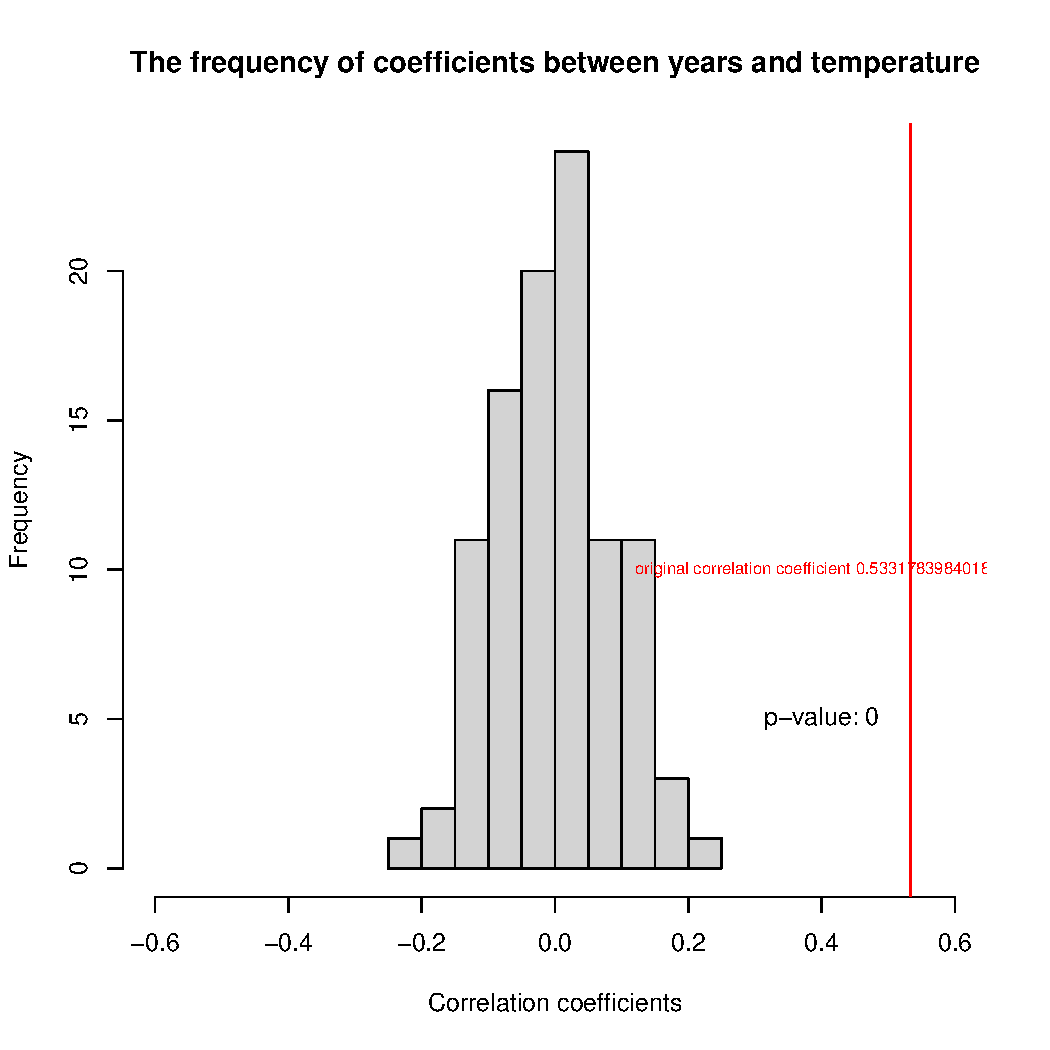
\includegraphics[scale = 0.7]{../data/Floridaplot.pdf}
\end{center}
\section{Interpretation}
To ensure the variables are independent, a permutation analysis is conducted by randomly reshuffling the temperatures and calculate the coefficients. The distribution of the calculated coefficients are shown in the results graph, and is compared to the original correlation coefficient, which is shown to be approximately 0.533.
\bigbreak
\noindent According to our result, the p-value is 0 since there is no random correlation coefficient detected which is greater than the observed value, 0.533. It is also noticeable that the original correlation coefficient is much larger than the maximum value from the distribution. This indicates a strong evidence to reject the null hypothesis of no significant correlation between the temperature and year. In this case, we can conclude that the temperature in Florida is correlated with the year.

\end{document}  
